%\documentclass[sfsidenotes]{tufte-book}
\documentclass[phd,lfcs,notimes,openright]{infthesis}
\usepackage{phdthesis}
\usepackage{subfiles}

\title{Formally Describing Informal Policies in the Mobile Ecosystem}
\author{Joseph Hallett}
\submityear{2017}
\abstract{TODO}

\begin{document}
\begin{preliminary}
  \maketitle
  \begin{acknowledgements}
    I am grateful to many people for their help in completing my PhD.  In particular I would like to thank the following people:
    
    Thankyou to my supervisors David Aspinall and Bj\"orn Franke for their advice, criticism, help, patience, and always offering to edit my papers.
    Thankyou to Andy Gordon and Martin Hofmann for the helpful discussions early on, introducing me to SecPAL and to using formal logic to model this domain.
    Thankyou to Daniel Franzen, Marcin Szymczak, Arthur Chan, Catherine Crompton and the rest of IF~5.24 for listening to my rants and helpful discussions over the years.
    Thankyou to Dan Page for his help early in my career, and for suggesting I apply for this job.
    A second thankyou to David Aspinall for helping me move back home to be a proper father to my son, before I really should have and for sorting out the paperwork when the university eventually noticed.
    Thankyou to my friends and family for supporting me over the past years, especially Di for her camaraderie in completing this.
    Thankyou to EasyJet for roughly 307 safe flights between Ediburgh and Bristol (and one slightly terrifying one). 

    Finally, thankyou to Emma and Jim. 
    Thankyou Emma for your unwaivering support and for letting me work when I should be helping with the baby, and thankyou Jim for keeping me awake and writing at all hours.
    

  \end{acknowledgements}
  \standarddeclaration{}
  \dedication{
    This thesis is dedicated to Emma, for putting up with me.

    \vspace{8em}
    {\itshape
      ``You cannot have a secure Android phone for two reasons: 1) it is Android, 2) it is a phone. 
      step 1, get google out of it.  Step 2, everything else'' --- \emph{The Grugq}

    \vspace{2em}

      ``It's too late to fire you, you better get a PhD'' --- \emph{David Aspinall}
    }
  }
  \tableofcontents
  \listoffigures
  \listoftables
\end{preliminary}

\subfile{chapters/01-introduction.tex}
\subfile{chapters/02-background.tex}
\subfile{chapters/03-apppal.tex}
\subfile{chapters/04-apps-and-app-stores.tex}
\subfile{chapters/05-reasoning-about-policies.tex}
\subfile{chapters/future-work.tex}
\subfile{chapters/06-related-work.tex}
\subfile{chapters/07-conclusion.tex}

\appendix
\chapter{Translated BYOD Policies}
\label{appendix:byod}
\section{NHS}
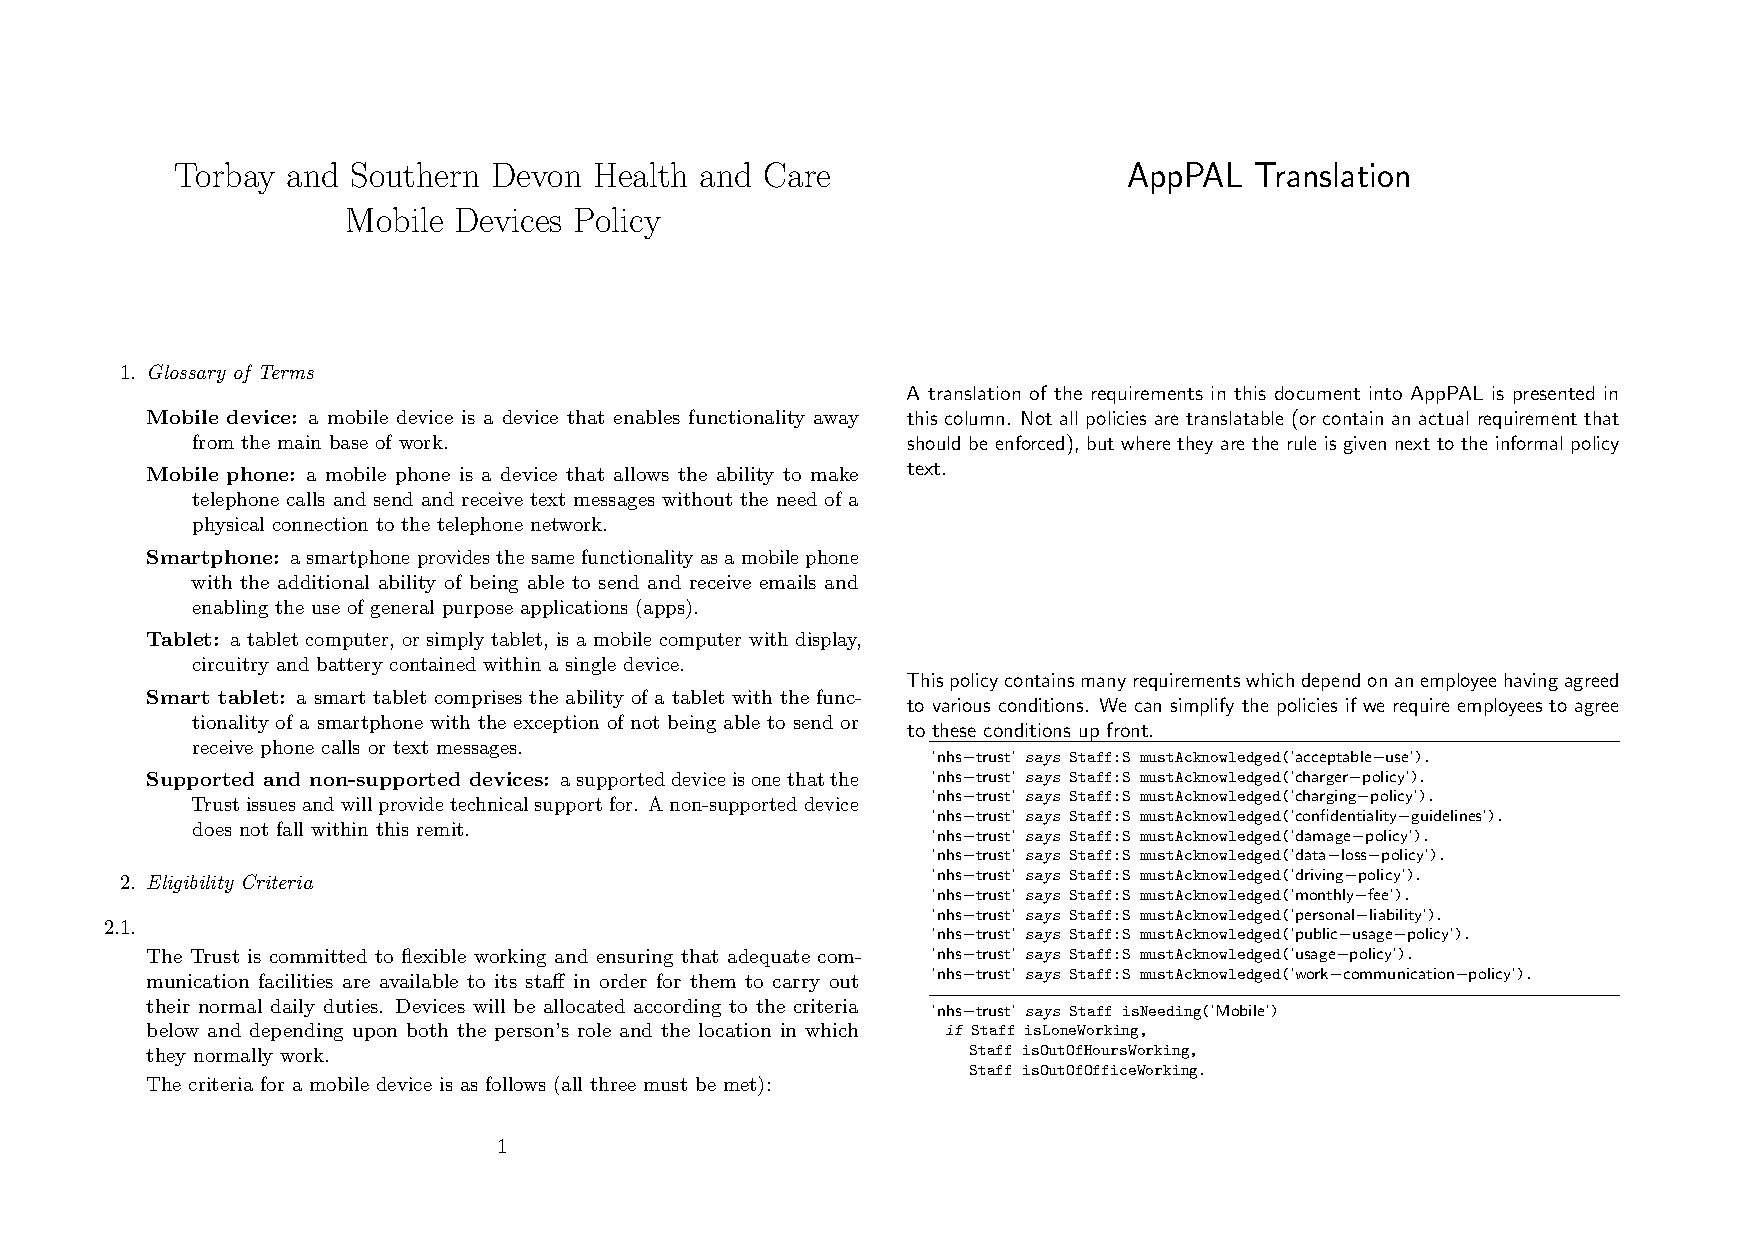
\includepdf[pages={-},landscape]{appendixes/nhs.pdf}
\section{SANS}
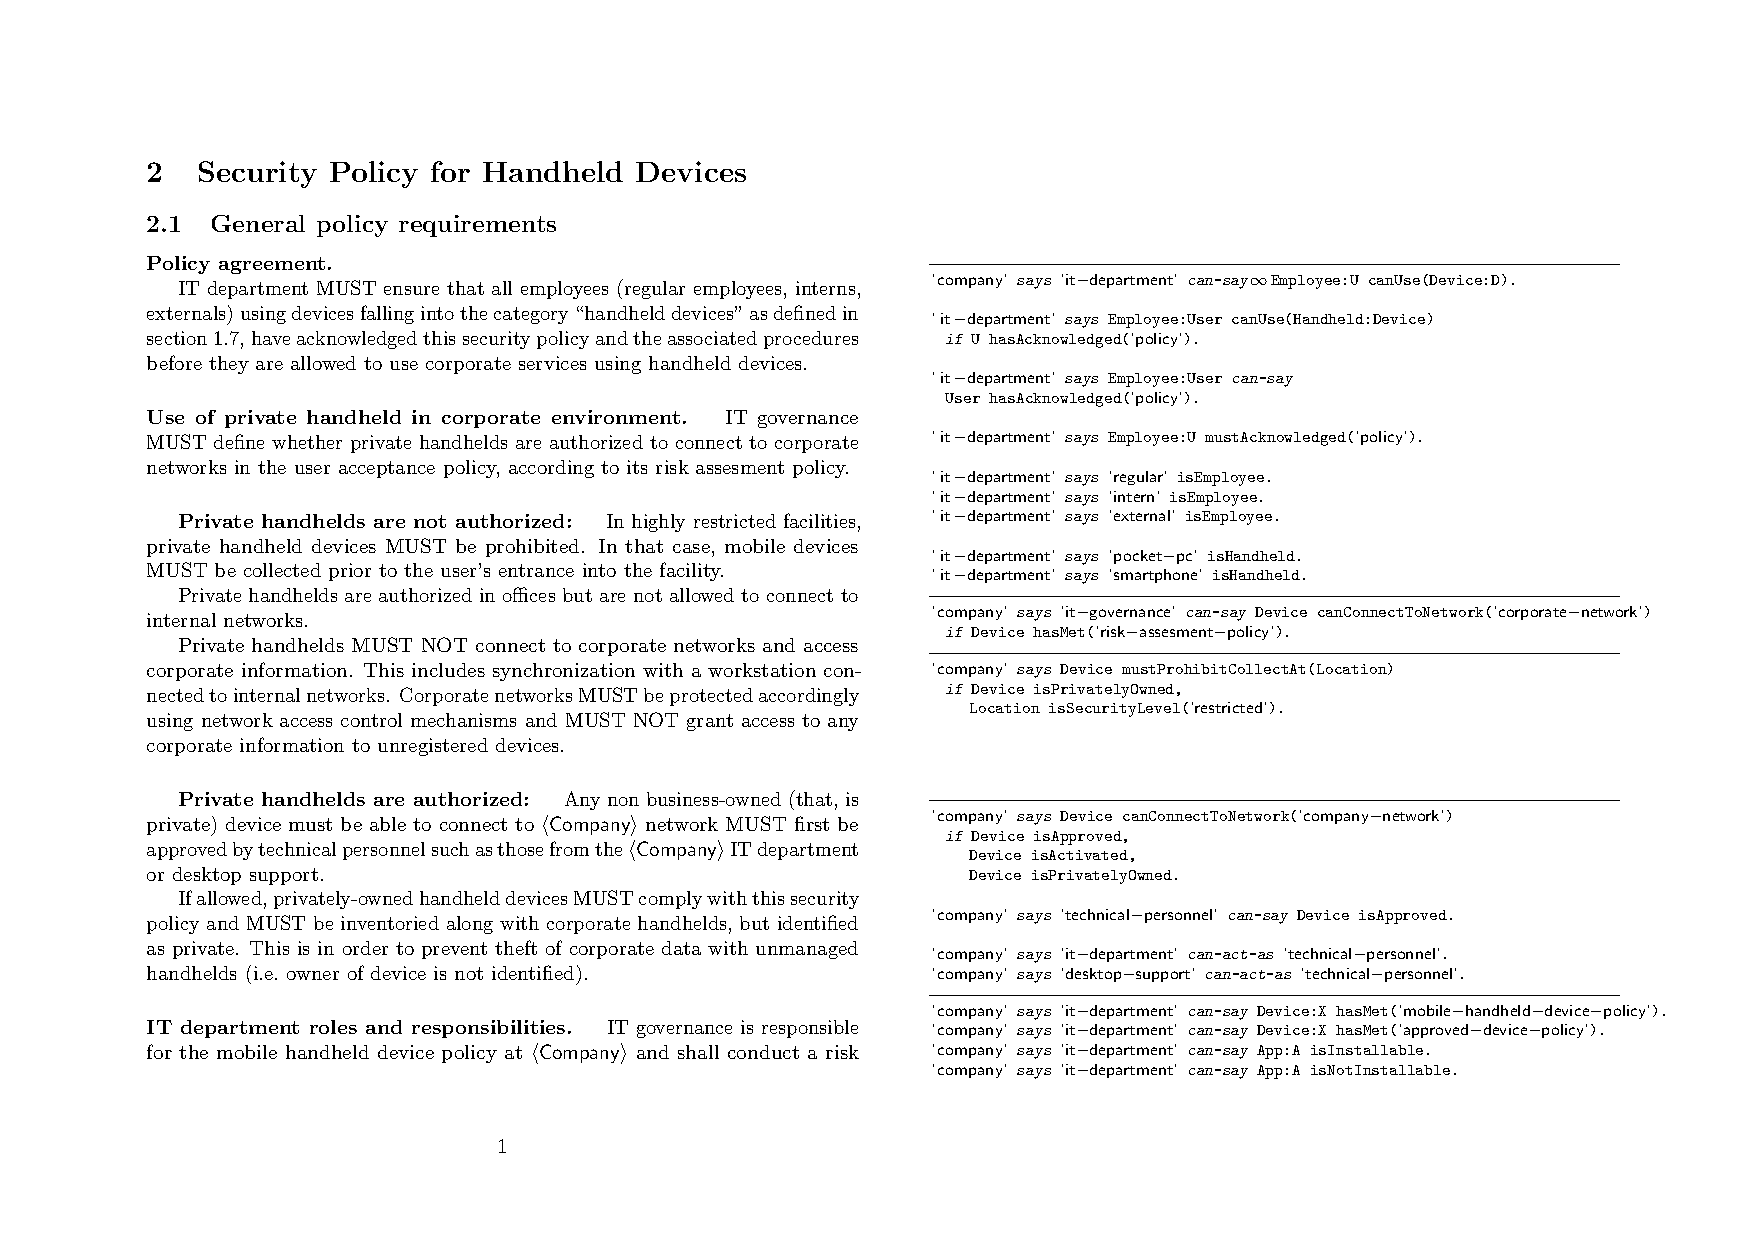
\includepdf[pages={-},landscape]{appendixes/sans.pdf}
\section{HiMSS}
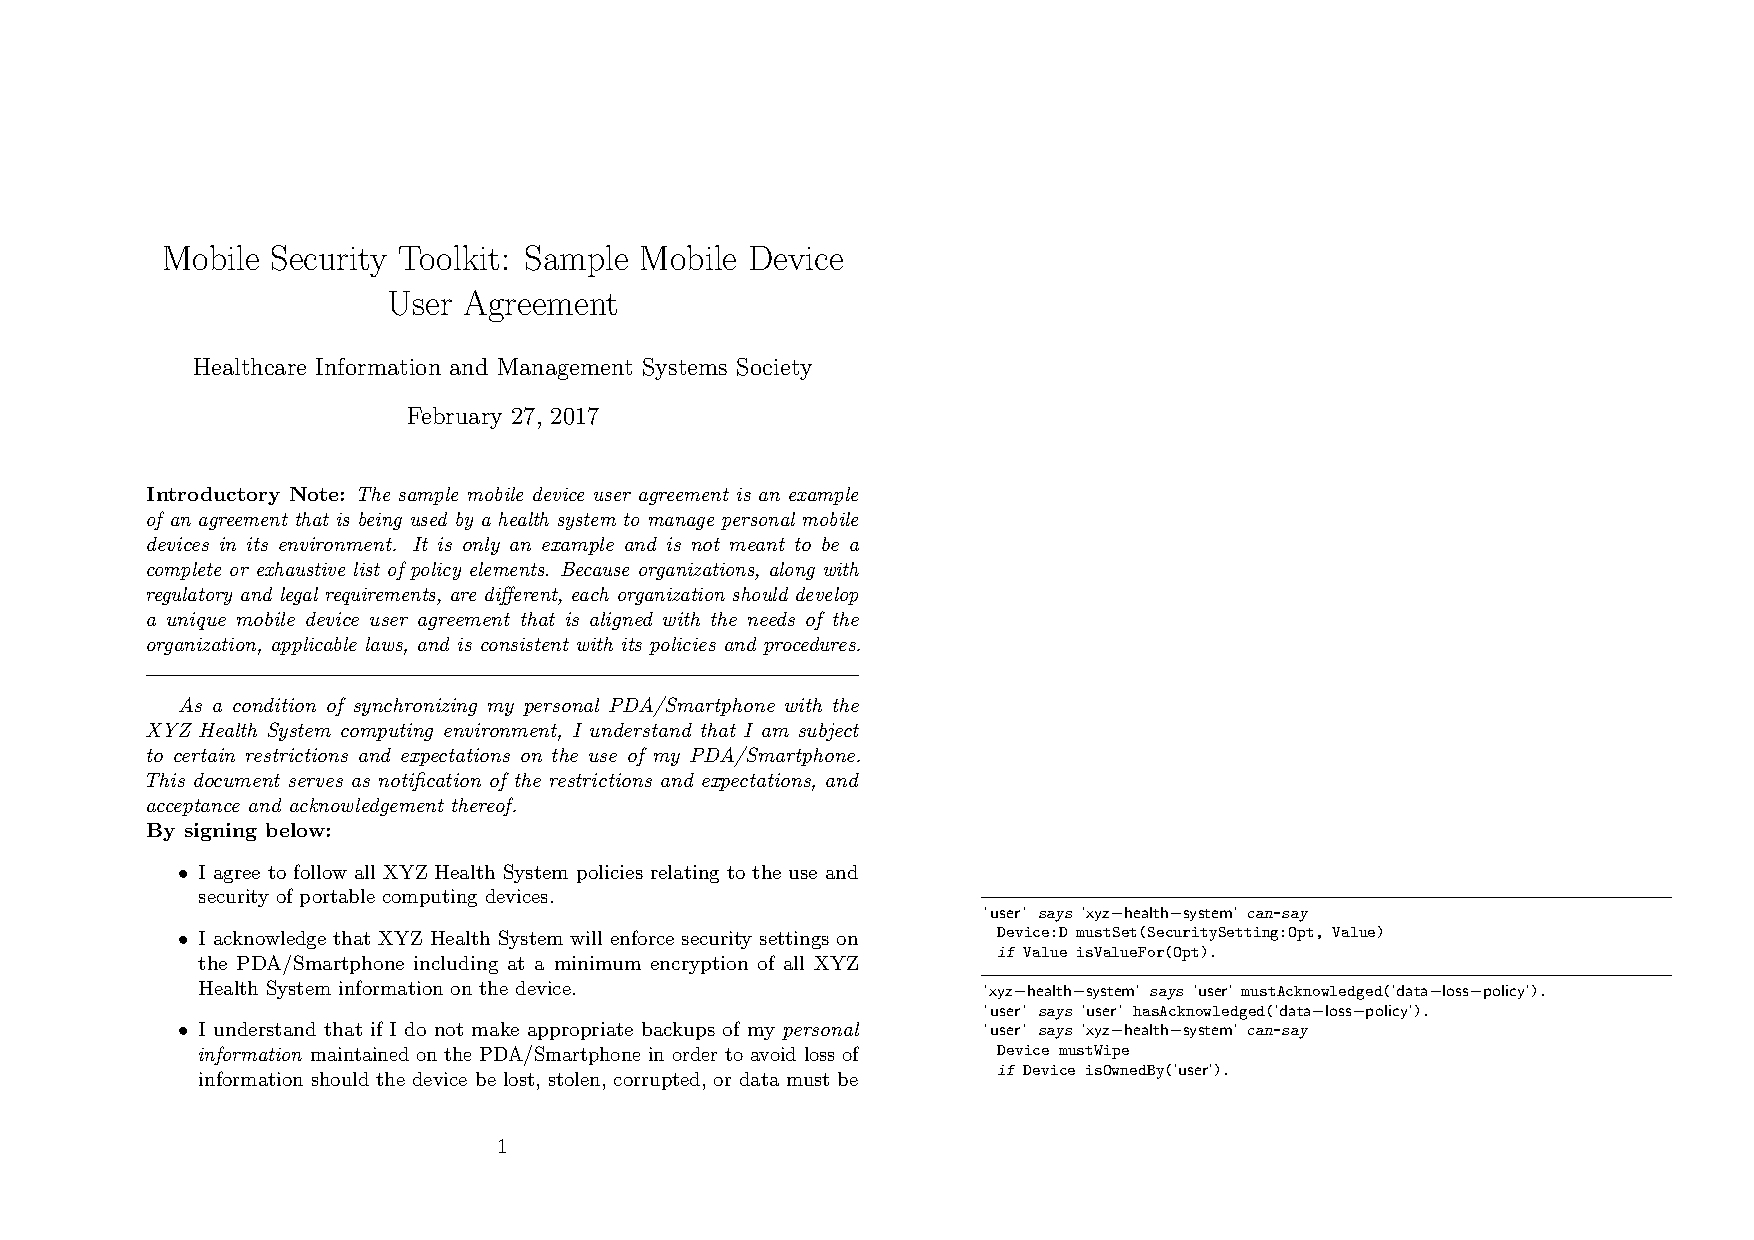
\includepdf[pages={-},landscape]{appendixes/himss.pdf}
\section{Edinburgh}
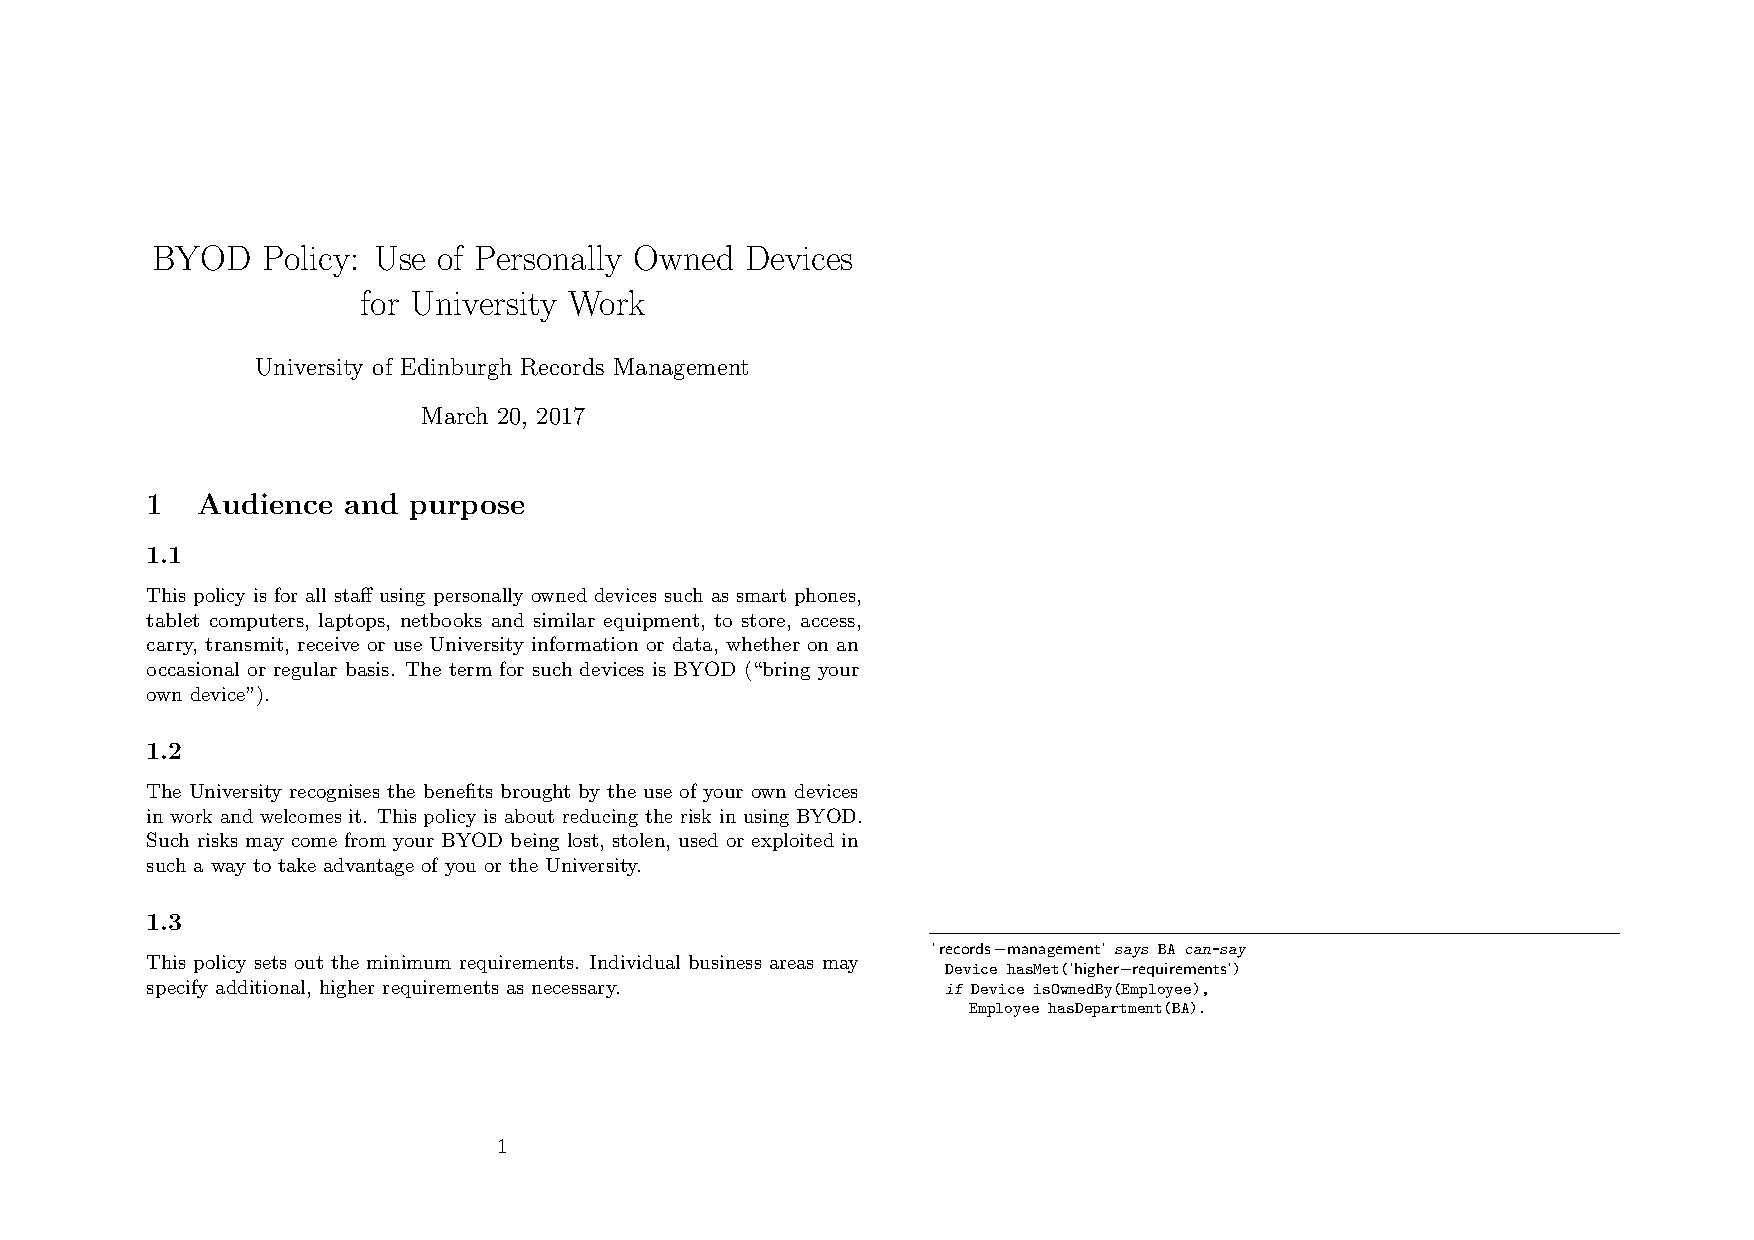
\includepdf[pages={-},landscape]{appendixes/edinburgh.pdf}
\section{Sirens}
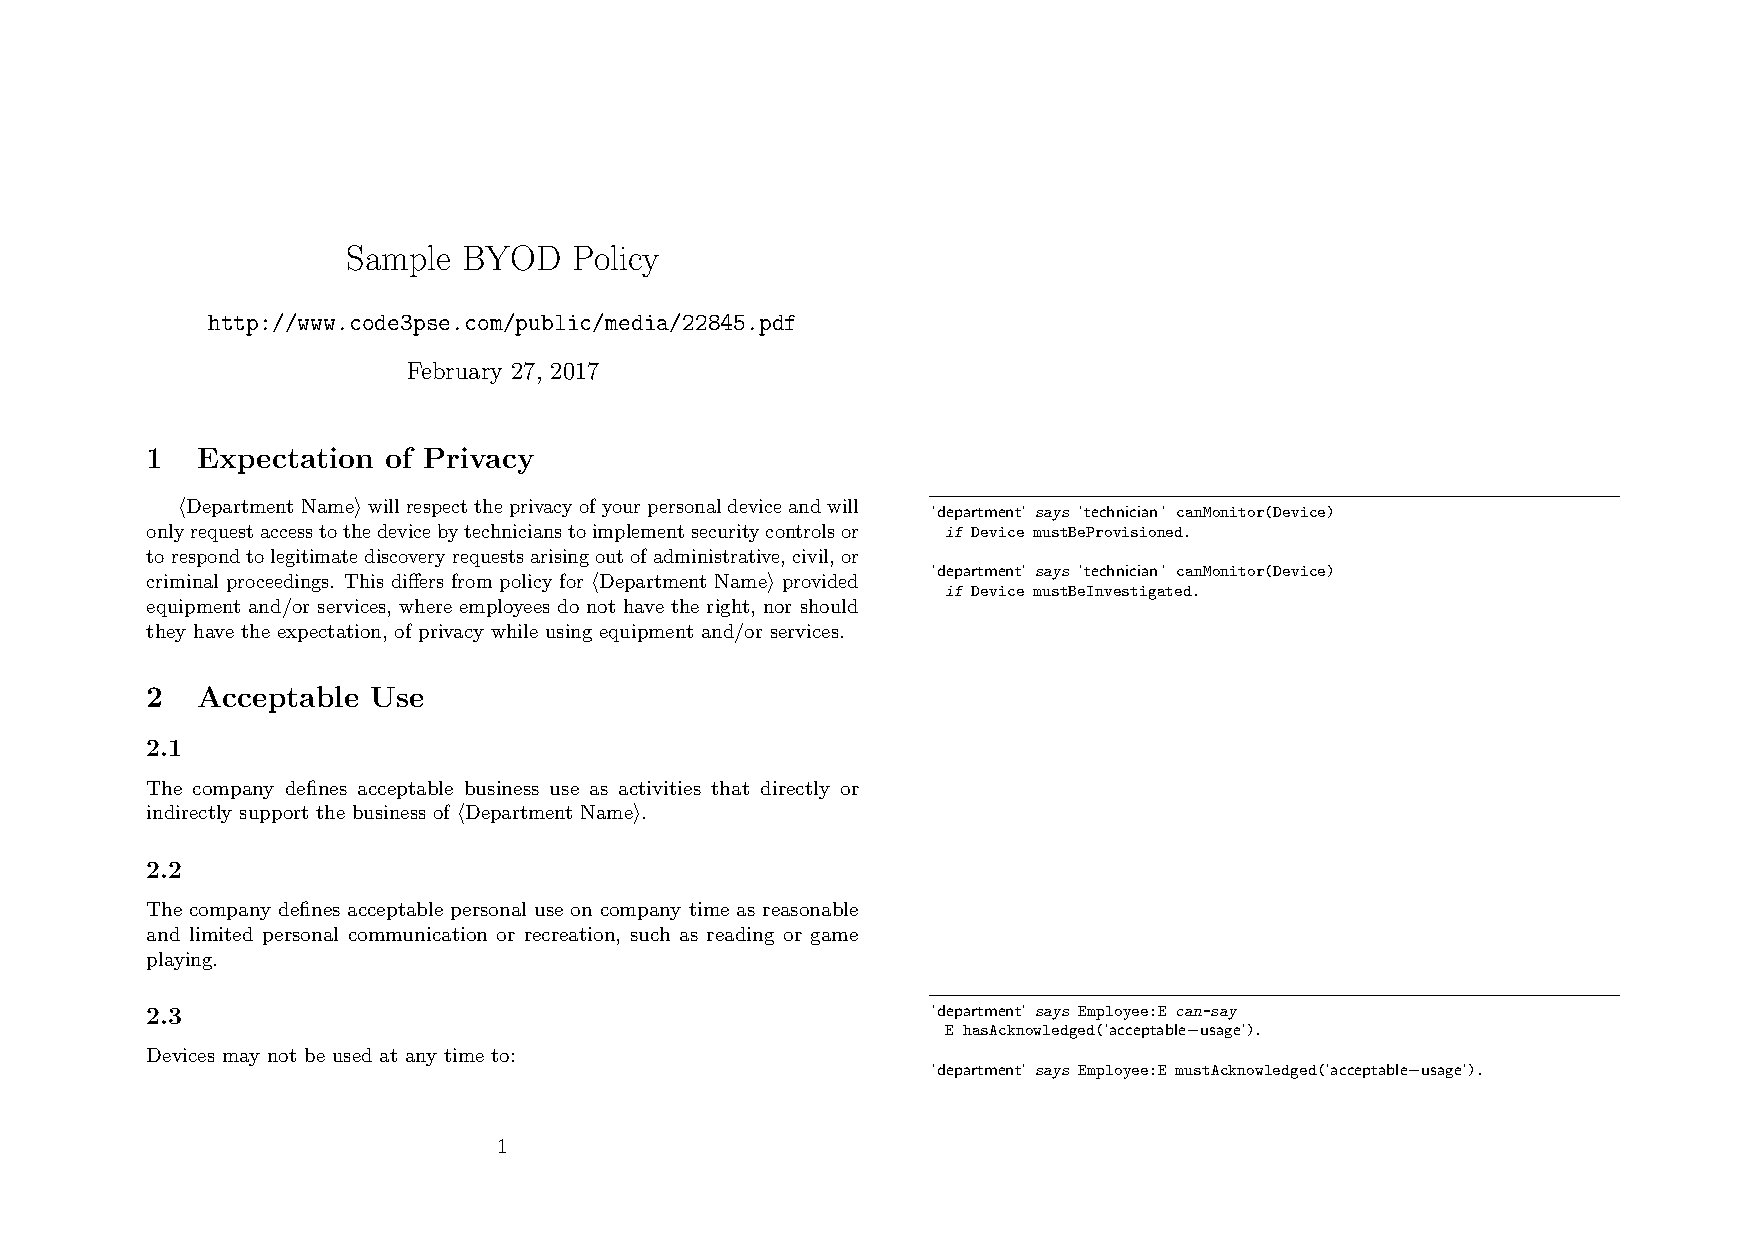
\includepdf[pages={-},landscape]{appendixes/code3pse.pdf}

\subfile{chapters/appendix-secpal-to-datalogc.tex}

%\bibliographystyle{plainnat}
\singlespace
\bibliographystyle{plain}
\bibliography{thesis}

\end{document}

%%% Local Variables:
%%% mode: latex
%%% TeX-master: t
%%% End:
